\documentclass{beamer}[10]

\usepackage{graphicx}
\usepackage{xcolor}
\usepackage{tabto}
%\usepackage{beamerthemesplit}
\usepackage{tikz}
\usepackage{cancel}
\usepackage{verbatim}
\usepackage{fancybox}
\usepackage{enumerate}
\usepackage{amsmath,amssymb,amsthm,textcomp,mathtools}
\usepackage[super]{nth}
\usepackage[amssymb]{SIunits}
\usepackage{booktabs}
\usepackage{cancel}
\usepackage{bm}
\usepackage[utf8]{inputenc}
\usepackage{tabularx}
\usepackage{ragged2e}
\newcolumntype{Y}{ >{\RaggedRight\arraybackslash}X}
\usetikzlibrary{arrows,shapes}
\newcommand\T{\rule{0pt}{2.6ex}}
\newcommand\B{\rule[-1.2ex]{0pt}{0pt}}
\definecolor{UUcrimson}{RGB}{204,0,0}
\mode<presentation>
{ \usetheme{default}
  \usecolortheme[named=UUcrimson]{structure}
  \useinnertheme{circles}
  \setbeamercovered{transparent}
  \setbeamertemplate{blocks}[rounded]
  \usefonttheme[onlymath]{serif}
  \setbeamertemplate{navigation symbols}{}
  \setbeamertemplate{footline}[page number]
  \setbeamertemplate{navigation symbols}{}
  \setbeamercolor{section in toc}{fg=black,bg=white}
  \setbeamercolor{alerted text}{fg=UUcrimson!80!gray}
  \setbeamercolor*{palette primary}{fg=white,bg=UUcrimson}
  \setbeamercolor*{palette secondary}{fg=UUcrimson!70!black,bg=gray!15!white}
  \setbeamercolor*{palette tertiary}{bg=UUcrimson!80!black,fg=gray!10!white}
  \setbeamercolor*{palette quaternary}{fg=UUcrimson,bg=gray!5!white}
  \setbeamercolor*{palette sidebar primary}{fg=UUcrimson!10!black}
  \setbeamercolor*{palette sidebar secondary}{fg=white}
  \setbeamercolor*{palette sidebar tertiary}{fg=UUcrimson!50!black}
  \setbeamercolor*{palette sidebar quaternary}{fg=gray!10!white}
  \setbeamercolor{titlelike}{parent=palette primary,fg=white}
  \setbeamercolor{frametitle}{bg=UUcrimson}
  \setbeamercolor{frametitle right}{bg=UUcrimson}
  \setbeamercolor*{separation line}{}
  \setbeamercolor*{fine separation line}{}
}

\usetikzlibrary{backgrounds}
\makeatletter
\tikzstyle{every picture}+=[remember picture]
\tikzset{%
  fancy quotes/.style={
    text width=\fq@width pt,
    align=justify,
    inner sep=1em,
    anchor=north west,
    minimum width=\linewidth,
    font=\itshape
  },
  fancy quotes width/.initial={.8\linewidth},
  fancy quotes marks/.style={
    scale=8,
    text=white,
    inner sep=0pt,
  },
  fancy quotes opening/.style={
    fancy quotes marks,
  },
  fancy quotes closing/.style={
    fancy quotes marks,
  },
  fancy quotes background/.style={
    show background rectangle,
    inner frame xsep=0pt,
    background rectangle/.style={
      fill=gray!25,
      rounded corners,
    },
  }
}
\newenvironment{fancyquotes}[1][]{%
\noindent
\tikzpicture[fancy quotes background]
\node[fancy quotes opening,anchor=north west] (fq@ul) at (0,0) {``};
\tikz@scan@one@point\pgfutil@firstofone(fq@ul.east)
\pgfmathsetmacro{\fq@width}{\linewidth - 2*\pgf@x}
\node[fancy quotes,#1] (fq@txt) at (fq@ul.north west) \bgroup}
{\egroup;
\node[overlay,fancy quotes closing,anchor=east] at (fq@txt.south east) {''};
\endtikzpicture}
\makeatother


\usetikzlibrary{backgrounds}
\makeatletter
\tikzstyle{every picture}+=[remember picture]
\tikzset{%
  fancy defs/.style={
    text width=\fq@width pt,
    align=justify,
    inner sep=0.25em,
    anchor=north west,
    minimum width=\linewidth,
    font=\itshape
  },
  fancy defs width/.initial={.8\linewidth},
  fancy defs marks/.style={
    scale=8,
    text=white,
    inner sep=0pt,
  },
  fancy defs opening/.style={
    fancy defs marks,
  },
  fancy defs closing/.style={
    fancy defs marks,
  },
  fancy defs background/.style={
    show background rectangle,
    inner frame xsep=0pt,
    background rectangle/.style={
      fill=gray!25,
      rounded corners,
    },
  }
}
\newenvironment{fancydefs}[1][]{%
\noindent
\tikzpicture[fancy defs background]
\node[fancy defs opening,anchor=north west] (fq@ul) at (0,0) {};
\tikz@scan@one@point\pgfutil@firstofone(fq@ul.east)
\pgfmathsetmacro{\fq@width}{\linewidth - 2*\pgf@x}
\node[fancy defs,#1] (fq@txt) at (fq@ul.north west) \bgroup}
{\egroup;
\node[overlay,fancy defs closing,anchor=east] at (fq@txt.south east) {};
\endtikzpicture}
\makeatother
\usepackage{scalerel}[2014/03/10]
\usepackage{stackengine}
\usepackage{empheq}
\newcommand*\widefbox[1]{\fbox{\hspace{0.5em}#1\hspace{0.5em}}}

\newcommand\reallywidetilde[1]{\ThisStyle{%
  \setbox0=\hbox{$\SavedStyle#1$}%
  \stackengine{-.1\LMpt}{$\SavedStyle#1$}{%
    \stretchto{\scaleto{\SavedStyle\mkern.2mu\sim}{.5467\wd0}}{.4\ht0}%
%    .2mu is the kern imbalance when clipping white space
%    .5467++++ is \ht/[kerned \wd] aspect ratio for \sim glyph
  }{O}{c}{F}{T}{S}%
}}
\usepackage{media9}

\logo{
\includegraphics[width=0.75cm]{logo.jpg}}
\author[Gibbs]{Dr. Jeremy A. Gibbs}
\institute{Department of Mechanical Engineering\\University of Utah}
\date{Spring 2017}
\title{Environmental Fluid Dynamics: Lecture 8}
% colors
\definecolor{colororange}{HTML}{E65100} % orange
\definecolor{colordgray}{HTML}{795548} % dark gray for note
\definecolor{colorhgray}{HTML}{212121} % heavy dark gray for normal text
\definecolor{colorgreen}{HTML}{009688} % green
\definecolor{colorwhite}{HTML}{FFFFFF} % background white
\definecolor{colorlgray}{HTML}{F5F3EE} % background light gray
\definecolor{colorblue}{HTML}{0277BB} % blue
\definecolor{colorred}{HTML}{CC0000} % red
\usepackage{esvect}
\newcommand{\fontsizeone}{1.9em}
\setbeamertemplate{caption}{\raggedright\insertcaption\par}
\newcommand{\framecard}[2][colorgreen]{
  {\setbeamercolor{background canvas}{bg=#1}
    \begin{frame}[plain]
    \vfill
    \begin{center}
     {#2}
    \end{center}
    \vfill
    \end{frame}
  }
}
\begin{document}

%----------------------------------------------------------------------------------------
%	TITLE & TOC SLIDES
%----------------------------------------------------------------------------------------

\begin{frame} 
  \titlepage
\end{frame}

%------------------------------------------------

\begin{frame}
\frametitle{Overview}
\tableofcontents
\end{frame}

%------------------------------------------------
\section{Atmospheric Dynamics: Basic Equations} %
%------------------------------------------------
\subsection{Overview}
%------------------------------------------------
\begin{frame}{Basic Equations of Fluid Dynamics}

\begin{itemize}
	\item We are interested in the basic equations of fluids dynamics applied to the atmosphere (i.e., a rotating coordinate system)
	\item These include
	\begin{itemize}
		\item Conservation of Mass
		\item Conservation of Momentum
		\item Conservation of Energy (mechanical and total)
	\end{itemize}
	\item In general, we would like to determine the transport of mass, momentum, energy, or scalars
	\item We will present these in differential, Eulerian form
\end{itemize}
\end{frame}
%------------------------------------------------
\subsection{Review: Lagrangian vs. Eulerian}
%------------------------------------------------
\framecard[colorred]{{\color{white}\Huge Review:\\~\\Lagrangian vs. Eulerian}}
%------------------------------------------------
\begin{frame}{Review: Lagrangian vs. Eulerian}

\textbf{Lagrangian}
\begin{itemize}
	\item Description of how quantities change with time for an air parcel (following air parcel motion).
	\item $x(t), y(t), z(t)$ are Cartesian coordinates of the position of the parcel and are dependent variables.
	\item $t$ is an independent variable.
	\item $\vv{r}(t) \equiv x(t)\hat i + y(t) \hat j + z(t) \hat k$ is the parcel position vector.
	\item $\frac{D()}{DT}$ is the rate of change of $()$.
	\item $\frac{D}{DT}$ is the (total, substantial, particle, individual, Lagrangian, material) operator.
\end{itemize}
\end{frame}
%------------------------------------------------
\begin{frame}{Review: Lagrangian vs. Eulerian}

\textbf{Lagrangian}
\begin{itemize}
	\item For velocity:
	$$\vv{u} \equiv \frac{D\vv{r}}{Dt} = \frac{Dx}{Dt}\hat i + \frac{Dy}{Dt}\hat j + \frac{Dz}{Dt}\hat k = u \hat i + v\hat j + w\hat k$$
	\item The acceleration is:
	$$\vv{a} \equiv \frac{D\vv{u}}{Dt}$$
	\item Thus, 
	$$\vv{F} = m\vv{a} = m\frac{D\vv{u}}{Dt} = m\frac{D^2 \vv{r}}{Dt^2}$$
\end{itemize}
\end{frame}
%------------------------------------------------
\begin{frame}{Review: Lagrangian vs. Eulerian}

\textbf{Eulerian}
\begin{itemize}
	\item Description of how quantities change with time at a fixed point in space (not following parcel).
	\item $T(x,y,z,t)$ is temperature at a point ($x,y,z$) in space at time $t$.
	\item Here, $x,y,z,t$ are independent variables.
	\item $\frac{\partial T}{\partial t}$ is the local derivative of $T$ - the time rate of change of $T$ at a fixed point.
	\item Generally, $D/Dt \neq \partial /\partial t$, but they are related
\end{itemize}
\end{frame}
%------------------------------------------------
\begin{frame}{Review: Lagrangian vs. Eulerian}

\textbf{Relationship Between Lagrangian and Eulerian}
\begin{itemize}
	\item At time $t_0$, a parcel of air is at $x_0, y_0, z_0$ with temperature:
	\begin{itemize}
		\item Lagrangian: $T(t_0)$
		\item Eulerian: $T(x_0, y_0, z_0,t_0)$
	\end{itemize}
	\item Let's consider the parcel at time $t=t_0+\delta t$.
	\begin{itemize}
	\item Lagrangian: $T=T(t_0+ \delta t)$
	\item Eulerian: $T=T(x_0+\delta x, y_0+\delta y, z_0+\delta z,t_0+ \delta t)$
	\end{itemize}
	\item Time change in the Lagrangian viewpoint is:
	$$\frac{DT}{Dt} = \lim_{\delta t\rightarrow 0} \frac{T(t_0 + \delta t) - T(t_0)}{\delta t}$$
	\item Expand the right-hand side using the Eulerian viewpoint:
	$$\frac{DT}{Dt} = \lim_{\delta t\rightarrow 0} \frac{T(x_0+\delta x, y_0+\delta y, z_0+\delta z,t_0+ \delta t) - T(x_0, y_0, z_0,t_0)}{\delta t}$$
\end{itemize}
\end{frame}
%------------------------------------------------
\begin{frame}{Review: Lagrangian vs. Eulerian}

\textbf{Relationship Between Lagrangian and Eulerian}
\begin{itemize}
	\item Now we apply the Taylor expansion and neglect higher-order terms.
	\begin{align*}
		\frac{DT}{Dt} &= \lim_{\delta t\rightarrow 0}\frac{T_0 + \frac{\partial T}{\partial x}\delta x + \frac{\partial T}{\partial y}\delta y + \frac{\partial T}{\partial z}\delta z + \frac{\partial T}{\partial t}\delta t - T_0}{\delta t}\\
		&= \lim_{\delta t\rightarrow 0} \left(\frac{\partial T}{\partial x}\frac{\delta x}{\delta t} + \frac{\partial T}{\partial y}\frac{\delta y}{\delta t} + \frac{\partial T}{\partial z}\frac{\delta z}{\delta t} + \frac{\partial T}{\partial t} \right)\\
		&= \frac{\partial T}{\partial t} + u\frac{\partial T}{\partial x} + v\frac{\partial T}{\partial y} + w\frac{\partial T}{\partial z}
	\end{align*}
	where $$T_0 = T(x_0, y_0, z_0,t_0)$$ and $$u=\lim_{\delta t\rightarrow 0} \frac{\delta x}{\delta t}, v=\lim_{\delta t\rightarrow 0} \frac{\delta y}{\delta t}, w=\lim_{\delta t\rightarrow 0} \frac{\delta z}{\delta t}$$
\end{itemize}
\end{frame}

%------------------------------------------------
\begin{frame}{Review: Lagrangian vs. Eulerian}

\textbf{Relationship Between Lagrangian and Eulerian}
\begin{itemize}
	\item So, we have:
	$$\underbrace{\frac{DT}{Dt}}_{\text{total deriv}} = \underbrace{\frac{\partial T}{\partial t}}_{\text{local deriv}} + \underbrace{u\frac{\partial T}{\partial x} + v\frac{\partial T}{\partial y} + w\frac{\partial T}{\partial z}}_{\text{advection terms}}$$
	or
	$$\frac{DT}{Dt} = \frac{\partial T}{\partial t} + \vv{u} \cdot \vv{\nabla} T$$
	\item In general,
	$$\frac{D()}{Dt} = \frac{\partial ()}{\partial t} + \vv{u} \cdot \vv{\nabla} ()$$
\end{itemize}
\end{frame}


%------------------------------------------------
\subsection{Conservation of Mass}
%------------------------------------------------
\framecard[colorred]{{\color{white}\Huge Atmospheric Dynamics:\\~\\Conservation of Mass}}
%------------------------------------------------
\begin{frame}{Conservation of Mass}

\begin{itemize}
	\item Consider a stationary volume of fluid through which mass is flowing - conceptually:\\
	\{mass accumulation rate\} = \{mass in rate\} - \{mass out rate\}
\end{itemize}
\begin{figure}
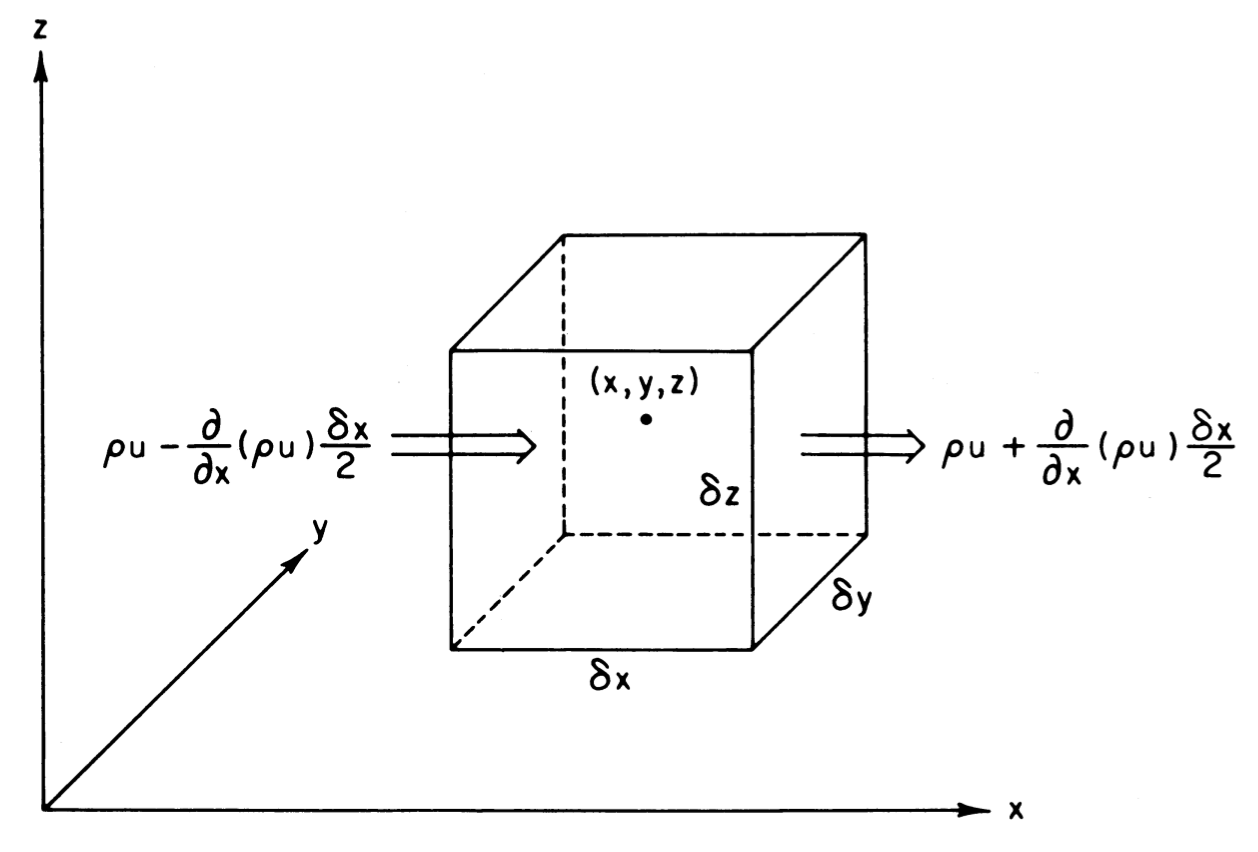
\includegraphics[width=0.8\textwidth]{fig1.png}\\
\centering \small From Holton (2004)
\end{figure}
\end{frame}
%------------------------------------------------
\begin{frame}{Conservation of Mass}

\begin{itemize}
	\item The rate of mass inflow through RHS
	$$\rho u - \frac{\partial (\rho u)}{\partial x}\frac{\delta x}{2}$$
	\item The rate of mass outflow through LHS
	$$\rho u + \frac{\partial (\rho u)}{\partial x}\frac{\delta x}{2}$$
	\item Note: area of each face is $\delta y \delta z$, so the net flow into the volume due to $u$ is
	$$\left[\rho u - \frac{\partial (\rho u)}{\partial x}\frac{\delta x}{2}\right]\delta y \delta z - \left[\rho u + \frac{\partial (\rho u)}{\partial x}\frac{\delta x}{2}\right]\delta y \delta z$$
	$$= -\frac{\partial (\rho u)}{\partial x} \delta x \delta y \delta z$$
\end{itemize}

\end{frame}

%------------------------------------------------
\begin{frame}{Conservation of Mass}

\begin{itemize}
	\item Similar expressions hold for the net mass flow into the volume due to $v$ and $w$, so that
	\begin{align*}
	\delta x \delta y \delta z \frac{\partial \rho}{\partial t} &= -\left[\frac{\partial (\rho u)}{\partial x} + \frac{\partial (\rho v)}{\partial y} + \frac{\partial (\rho w)}{\partial z}\right] \delta x \delta y \delta z\\
	\frac{\partial \rho}{\partial t} &= -\left[\frac{\partial (\rho u)}{\partial x} + \frac{\partial (\rho v)}{\partial y} + \frac{\partial (\rho w)}{\partial z}\right]\\
	\frac{\partial \rho}{\partial t} &= - \nabla \cdot (\rho \vv{U})
	\end{align*}
	Thus $$\boxed{\frac{\partial \rho}{\partial t} + \nabla \cdot (\rho \vv{U}) = 0}$$
	the \textbf{mass divergence form of the continuity equation}
	\end{itemize}
\end{frame}
%------------------------------------------------
\begin{frame}{Conservation of Mass}
$$\frac{\partial \rho}{\partial t} + \nabla \cdot (\rho \vv{U}) = 0$$
\begin{itemize}
	\item We can rewrite by using the following relationships
	\begin{align*}
	\nabla \cdot (\rho \vv{U}) &\equiv \rho \nabla \cdot \vv{U} + \vv{U} \cdot \nabla \rho\\
	\frac{D}{Dt} &\equiv \frac{\partial}{\partial t} + \vv{U} \cdot \nabla
	\end{align*}
	to arrive at
	\begin{align*}
		\frac{\partial \rho}{\partial t} + \rho \nabla \cdot \vv{U} + \vv{U} \cdot \nabla \rho &= 0\\
		\Aboxed{\frac{1}{\rho}\frac{D\rho}{Dt} + \nabla \cdot \vv{U} &= 0}
	\end{align*}
	the \textbf{velocity divergence form of the continuity equation}
\end{itemize}
\end{frame}

%------------------------------------------------
\begin{frame}{Conservation of Mass}
\textbf{mass divergence form of the continuity equation}
\begin{itemize}
	\item local rate of change of density is balanced by mass divergence
	$$\frac{\partial \rho}{\partial t} + \nabla \cdot (\rho \vv{U}) = 0$$
\end{itemize}
\textbf{velocity divergence form of the continuity equation}
\begin{itemize}
	\item the fractional rate of increase of density following the motion of an air parcel is balanced by the velocity divergence
	$$\frac{1}{\rho}\frac{D\rho}{Dt} + \nabla \cdot \vv{U} = 0$$
\end{itemize}
\end{frame}
%------------------------------------------------
\begin{frame}{Conservation of Mass: Incompressible Flow}
\begin{itemize}
	\item For many cases, the atmosphere may be considered incompressible
	\item \textbf{incompressible flow}: the density of a fluid element does not change during its motion (note: this \textit{does not} imply that density is constant everywhere)
	$$\frac{D\rho}{Dt} = 0$$
	thus, the continuity equation becomes
	$$\boxed{\nabla \cdot \vv{U} = 0}$$
\end{itemize}
\end{frame}
%------------------------------------------------
\begin{frame}{Conservation of Mass: Boussinesq Approximation}
\begin{itemize}
	\item We can extend the assumption of an incompressible flow and take the \textbf{Boussinesq approximation}
	\item Separate the density into 2 parts: a base state $\bar \rho (z)$ and perturbation $\rho^\prime$
	\item We will apply this after deriving an expression for the momentum balance equation
\end{itemize}
\end{frame}
%------------------------------------------------
\subsection{Conservation of Momentum}
%------------------------------------------------
\framecard[colorred]{{\color{white}\Huge Atmospheric Dynamics:\\~\\Conservation of Momentum}}
%------------------------------------------------
\begin{frame}{Conservation of Momentum}
\begin{itemize}
	\item Because the Earth's atmosphere has mass, we can apply Newton's \nth{2} Law
	$$\vv{F} = m \vv{a}$$
	where $\vv{F}$ is the sum of all forces acting on an object, $m$ is the mass of the object, and $\vv{a}$ is the acceleration of the object
	\item In classical mechanics, the object is usually some rigid solid body (\textit{e.g.}, ball, top, pendulum)
	\item In continuum mechanics, the object is usually some infinitesimal parcel of fluid or an elastic solid
	\item Since atmospheric dynamics is a branch of continuum mechanics, we will apply Newton's \nth{2} Law to a small volume element in the atmosphere
\end{itemize}
\end{frame}
%------------------------------------------------
\begin{frame}{Conservation of Momentum: Coordinate System}
\begin{itemize}
	\item We will apply Newton's \nth{2} Law to a rotating frame of reference. Why? Rotational effects are important for large-scale dynamics in the atmosphere.
	\item We choose a coordinate system that is fixed to the Earth, which is rotating. Why? That is where we make observations.
\end{itemize}
\end{frame}
%------------------------------------------------
\begin{frame}{Conservation of Momentum: Forces}
\begin{itemize}
	\item There are two categories of forces that we must consider: \textit{fundamental} and \textit{apparent}.
	\item \textbf{Fundamental Forces:} forces directly ``felt'' by the fluid.
	\item \textbf{Apparent Forces:} imaginary forces that result from acceleration of our coordinate system.
\end{itemize}
\end{frame}
%------------------------------------------------
\begin{frame}{Conservation of Momentum: In Words}
\begin{itemize}
	\item The conservation of momentum may be expressed in words as:
	\begin{align*}
	\left \{\parbox{5.4em}{\centering rate of\\ momentum\\accumulation}\right\} &= \left \{\parbox{5.4em}{\centering rate of\\momentum\\in}\right\} - \left \{\parbox{5.4em}{\centering rate of\\momentum\\out}\right\} \\&+ \left \{\parbox{5.4em}{\centering sum of\\fundamental\\forces}\right\} + \left \{\parbox{5.4em}{\centering sum of\\apparent\\forces}\right\}
	\end{align*}
\end{itemize}
\end{frame}
%------------------------------------------------
\begin{frame}{Conservation of Momentum: Fundamental Forces}
\begin{itemize}
	\item There are two types of fundamental forces in fluids: \textit{body} and \textit{surface}.
	\item \textbf{Body Forces:} the force on an object is proportional to the mass of
the object. This is often referred to as ``action at a distance'' (\textit{e.g.}, gravity, electromagnetic).
	\item \textbf{Surface Forces:} the force on an object is proportional to the surface area of the object. These forces are due to contact of the object with its surroundings, such as the force on the surface of a fluid element by an outside fluid (\textit{e.g.}, pressure, friction).
\end{itemize}
\end{frame}
%------------------------------------------------
\begin{frame}{Conservation of Momentum: Body Force (Gravity)}
\begin{itemize}
	\item Let's first derive an expression for the gravitational force, starting with Newton's law of gravitation:
	$$\vv{F_g} = -\frac{GMm}{r^2}\frac{\vv{r}}{r}$$
	which applies to two objects with masses $M$ and $m$, where $\vv{r}$ is the directed distance between their centers of mass, $r=|\vv{r}|$, and $G=6.67\times 10^{-11} \newton\  \metre\ \squared \kilo\gram\rpsquared$ is the universal gravitational constant.
\end{itemize}
\end{frame}
%------------------------------------------------
\begin{frame}{Conservation of Momentum: Body Force (Gravity)}
\begin{itemize}
	\item Let $\vv{r}$ point from a big object of mass $M$ to a little object of mass $m$. Then $\vv{F_g}$ is the gravitational force on $m$ due to $M$.
	\begin{figure}
		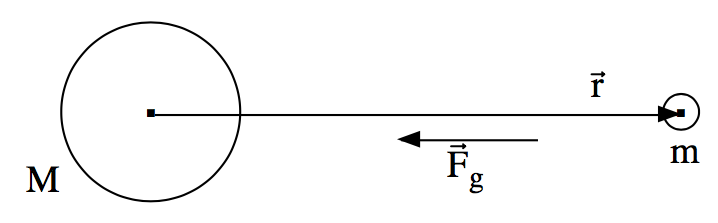
\includegraphics[width=0.8\textwidth]{gravity}	
	\end{figure}
	\item Let $\hat{r} \equiv \vv{r}/r$, so that $$\vv{F_g} = -\frac{GMm}{r^2}\hat{r},$$
	\item Thus, $|\vv{F_g}|$ is inversely proportional to the square of the distance between the the two masses (if $r\uparrow$ then $|\vv{F}_g|\downarrow$).
\end{itemize}
\end{frame}
%------------------------------------------------
\begin{frame}{Conservation of Momentum: Body Force (Gravity)}
\begin{itemize}
	\item Let $M$ be the mass of Earth and $m$ be the mass of a small parcel of air. We can then write the gravitational force per unit mass of air as:
	$$\underbrace{\frac{\vv{F_g}}{m}}_{\vv{g^*}}  = -\frac{GM}{r^2}\hat{r}$$
	\item Consider a parcel of air with mass $m$ at a height $z$ above Earth's surface in the troposphere
\end{itemize}
\end{frame}
%------------------------------------------------

\begin{frame}{Conservation of Momentum: Body Force (Gravity)}
  
\setlength{\fboxsep}{0pt}
\setlength{\fboxrule}{1pt}
\begin{columns}[T]
    \begin{column}{.58\textwidth}
    	\begin{itemize}
    		\item $a=6370\ \kilo\metre$ and $z<15\ \kilo\metre$
    		\item $r = a + z \approx a$, thus $r^2 \approx a^2$
    		\item $\vv{g^*} \approx -\frac{GM}{a^2} \hat{r}$ (in troposphere)
    		\item $M = \frac{4}{3} \pi a^3 \rho_e$, where $\rho_e = 5520\ \kilo\gram\ \second\rpsquared$ is the density of Earth
    		\item Thus, $\left|\vv{g^*}\right| \approx 9.8\ \metre\ \second\rpsquared$
    		\item This is gravitational acceleration
    	\end{itemize}	
    \end{column}
    \begin{column}{.42\textwidth}
    	\begin{minipage}[c][.4\textheight][c]{\linewidth}
    		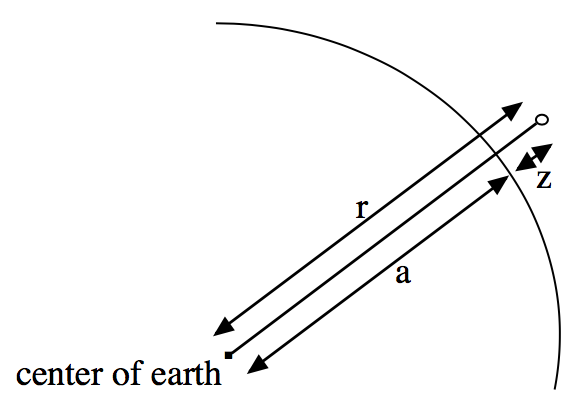
\includegraphics[width=\textwidth]{gravity2}
    	\end{minipage}
    \end{column}
  \end{columns}
\end{frame}
%------------------------------------------------
\begin{frame}{Conservation of Momentum: Surface Force (Pressure)}
\begin{itemize}
	\item Consider an infinitesimally small box of air with sides in the $x$, $y$, and $z$ directions of length $\delta x$, $\delta y$, and $\delta z$.
	\begin{figure}
		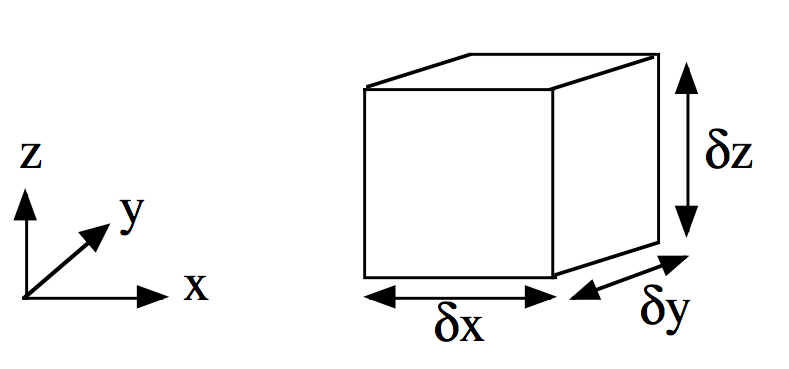
\includegraphics[width=0.8\textwidth]{pressure1.png}	
	\end{figure}
	\item We want to find the net pressure force on the box (note: pressure is a compressive force that acts perpendicular to the surfaces of the box)
\end{itemize}
\end{frame}
%------------------------------------------------
\begin{frame}{Conservation of Momentum: Surface Force (Pressure)}
\begin{itemize}
	\item Consider the $x$-component of the pressure force, (only include the two faces of the box perpendicular to the $x$-axis).
	\begin{figure}
		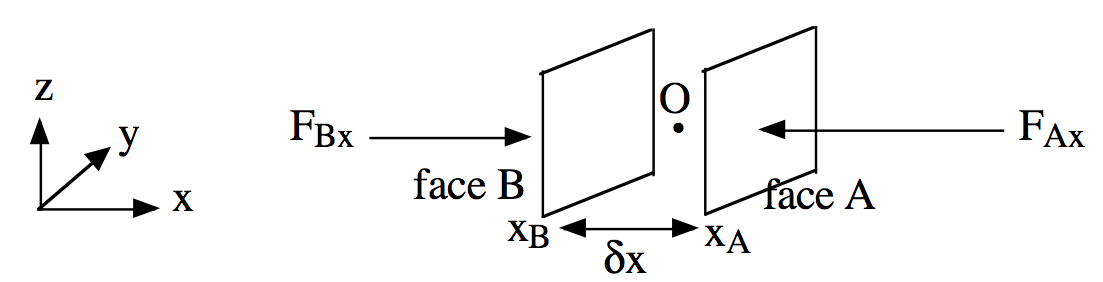
\includegraphics[width=0.8\textwidth]{pressure2.png}	
	\end{figure}
	\item Point 0 is at the center of the box, located at $x_0$, $y_0$, $z_0$.
	\item Pressure at center of box is $p_0$
	\item $F_{Ax}$ ($F_{bx}$) is the pressure force on face A (B) in $x$-direction.
	\item $X_A = x_0 + \delta x/2$, $X_B = x_0 - \delta x/2$
\end{itemize}
\end{frame}
%------------------------------------------------
\begin{frame}{Conservation of Momentum: Surface Force (Pressure)}
\begin{figure}
		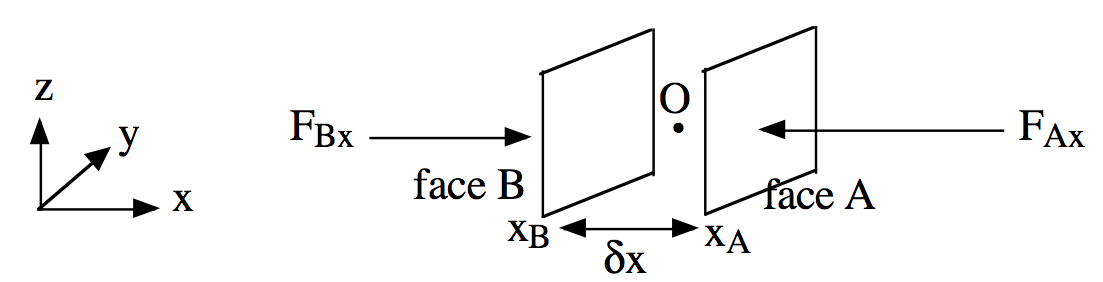
\includegraphics[width=0.75\textwidth]{pressure2.png}	
	\end{figure}
\begin{itemize}
	\item Using Taylor series, the pressure on face A is:
	\begin{align*}
	p_A &= p_0 + \left.\frac{\partial p}{\partial x}\right|_{x_0,y_0,z_0}(x_A - x_0) + \text{higher order terms (h.o.t.)}\\
	&= p_0 + \frac{\partial p}{\partial x} \left(x_0 + \frac{\delta x}{2} - x_0 \right)+ \cancelto{\text{very small}}{\text{h.o.t.}}\\
	&= p_0 + \frac{\partial p}{\partial x}\frac{\delta x}{2}
	\end{align*}
\end{itemize}
\end{frame}
%------------------------------------------------
\begin{frame}{Conservation of Momentum: Surface Force (Pressure)}
\begin{figure}
		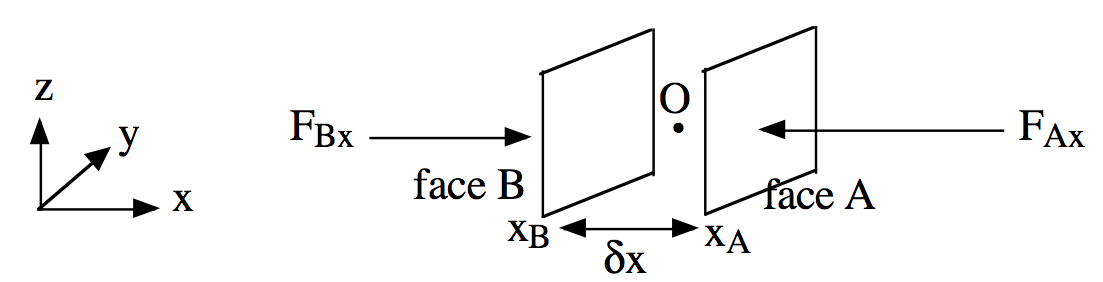
\includegraphics[width=0.75\textwidth]{pressure2.png}	
	\end{figure}
\begin{itemize}
	\item Pressure force (pressure $\times$ area) on face A is:
	\begin{align*}
	 	F_{Ax} &= -p_A \delta y \delta z\\
	 	&= -\left(p_0 + \frac{\partial p}{\partial x}\frac{\delta x}{2}\right)\delta y \delta z
	\end{align*}
	\item Note: the minus sign appears because the force exerted by the outside fluid on the inside fluid across face A is in the minus $x$-direction.
\end{itemize}
\end{frame}
%------------------------------------------------
\begin{frame}{Conservation of Momentum: Surface Force (Pressure)}
\begin{figure}
		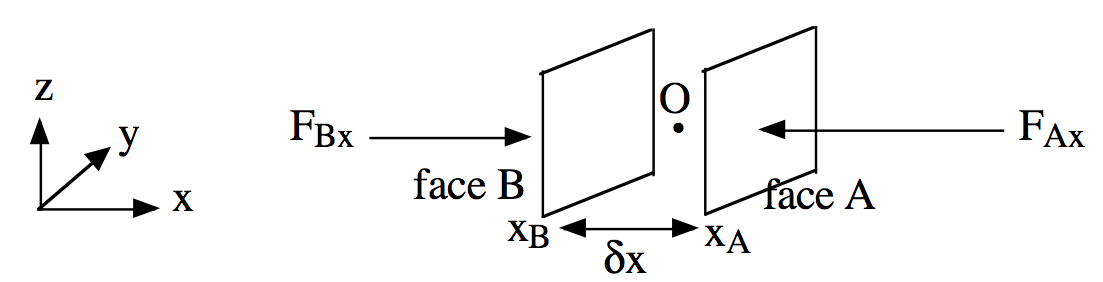
\includegraphics[width=0.75\textwidth]{pressure2.png}	
	\end{figure}
\begin{itemize}
	\item Using Taylor series, the pressure on face B is:
	\begin{align*}
	p_B &= p_0 + \left.\frac{\partial p}{\partial x}\right|_{x_0,y_0,z_0}(x_B - x_0) + \text{h.o.t.}\\
	&= p_0 + \frac{\partial p}{\partial x} \left(x_0 - \frac{\delta x}{2} - x_0 \right)+ \cancelto{\text{very small}}{\text{h.o.t.}}\\
	&= p_0 - \frac{\partial p}{\partial x}\frac{\delta x}{2}
	\end{align*}
\end{itemize}
\end{frame}
%------------------------------------------------
\begin{frame}{Conservation of Momentum: Surface Force (Pressure)}
\begin{figure}
		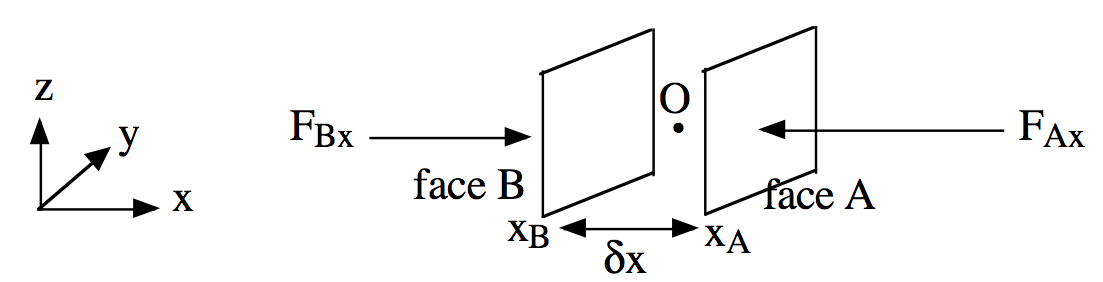
\includegraphics[width=0.75\textwidth]{pressure2.png}	
	\end{figure}
\begin{itemize}
	\item Pressure force (pressure*area) on face B is:
	\begin{align*}
	 	F_{Bx} &= p_B \delta y \delta z\\
	 	&= \left(p_0 - \frac{\partial p}{\partial x}\frac{\delta x}{2}\right)\delta y \delta z
	\end{align*}
\end{itemize}
\end{frame}
%------------------------------------------------
\begin{frame}{Conservation of Momentum: Surface Force (Pressure)}
\begin{figure}
		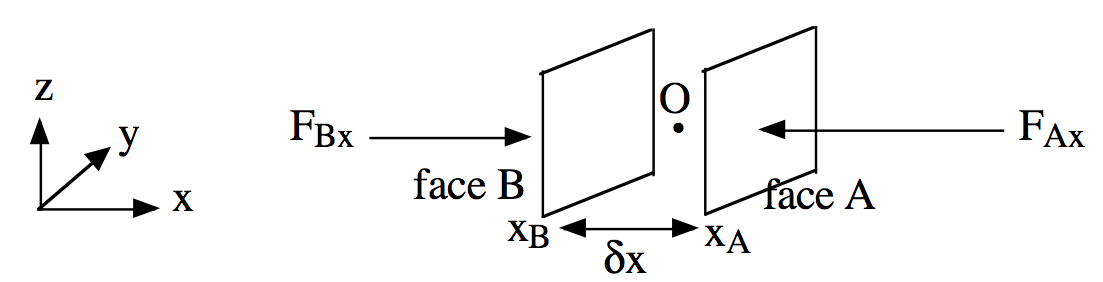
\includegraphics[width=0.75\textwidth]{pressure2.png}	
	\end{figure}
\begin{itemize}
	\item The net $x$-component pressure force on the box is:
	\begin{align*}
		F_x &\equiv F_{Ax} + F_{Bx}\\
		&= 	-\left(p_0 + \frac{\partial p}{\partial x}\frac{\delta x}{2}\right)\delta y \delta z + \left(p_0 - \frac{\partial p}{\partial x}\frac{\delta x}{2}\right)\delta y \delta z\\
		&= -\frac{\partial p}{\partial x}\delta x \delta y \delta z
	\end{align*}
	\item Thus, the net pressure on the box is proportional to the pressure gradient - the pressure gradient force (PGF).
\end{itemize}
\end{frame}
%------------------------------------------------
\begin{frame}{Conservation of Momentum: Surface Force (Pressure)}
\begin{itemize}
	\item If the mass of the box is $m=\rho \delta V = \rho \delta x \delta y \delta z$, then the $x$-component PGF per unit mass is:
	$$\frac{F_x}{m} = -\cfrac{\cfrac{\partial p}{\partial x}\delta x \delta y \delta z}{\rho \delta x \delta y \delta z} = -\frac{1}{\rho}\frac{\partial p}{\partial x}$$
	\item Similarly,
	$$\frac{F_y}{m} = -\frac{1}{\rho}\frac{\partial p}{\partial y} \qquad \text{and} \qquad \frac{F_z}{m} = -\frac{1}{\rho}\frac{\partial p}{\partial z}$$
	\item In vector form:
	$$\boxed{\frac{\vv{F_p}}{m} = -\frac{1}{\rho} \vv{\nabla} p}$$
\end{itemize}
\end{frame}
%------------------------------------------------
\begin{frame}{Conservation of Momentum: Surface Force (Pressure)}
$$\boxed{\frac{\vv{F_p}}{m} = -\frac{1}{\rho} \vv{\nabla} p}$$
\begin{itemize}
	\item Note: The PGF is proportional to the gradient of pressure and not the pressure itself.
	\item The magnitude of the PGF is large where the magnitude of $\vv{\nabla}p$ is large (tight isobars).
	\item The leading minus sign indicates that the PGF acts in the opposite direction of $\vv{\nabla}p$ (from high to low pressure).
\end{itemize}
\end{frame}
%------------------------------------------------
\begin{frame}{Conservation of Momentum: Surface Force (Friction)}
\begin{itemize}
	\item Now we consider the surface force due to molecular friction - the viscous force.
	\item To understand this force, consider fluid at rest between two infinite parallel plates. At time $t=0$ the top plate begins moving at a speed of $U_0$ in the $x$ direction:
	~\\~\\
	\begin{figure}
		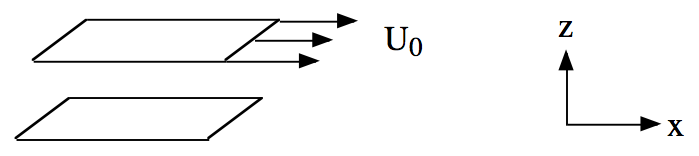
\includegraphics[width=0.8\textwidth]{friction1.png}
	\end{figure}
	\item The ``no-slip'' condition means that molecular friction causes fluid to stick to solid objects or boundaries.
\end{itemize}
\end{frame}
%------------------------------------------------
\begin{frame}{Conservation of Momentum: Surface Force (Friction)}
\begin{itemize}
	\item Fluid at the lower plate does not moves because it is sticking to the non-moving boundary.
	\item Fluid at the top plate moves at speed $U_0$ because it is sticking to the moving boundary.
	\begin{figure}
		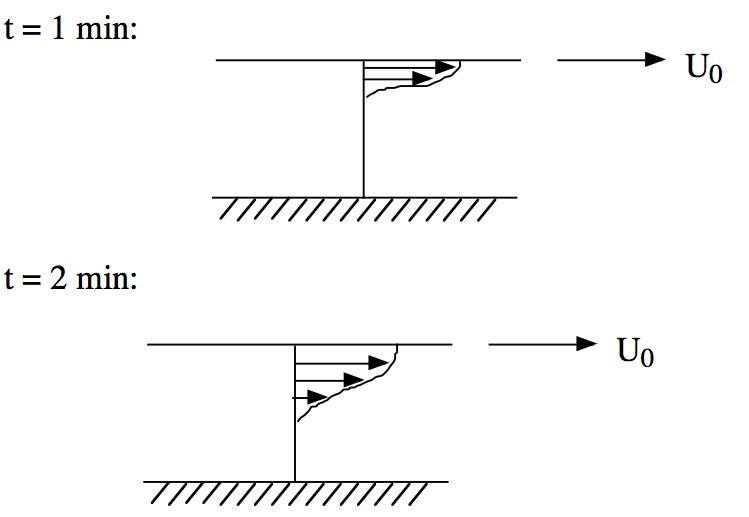
\includegraphics[width=0.8\textwidth]{friction2.png}
	\end{figure}
\end{itemize}
\end{frame}
%------------------------------------------------
\begin{frame}{Conservation of Momentum: Surface Force (Friction)}
\begin{itemize}
	\item Eventually we get a steady-state, where there is no change in velocity with time at any point.
	\item For this experiment, steady-state looks like:
	\begin{figure}
		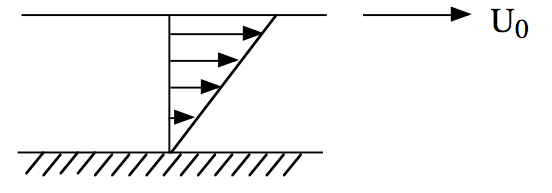
\includegraphics[width=0.8\textwidth]{friction3.png}
	\end{figure}
	\item We find that $u = U_0 \frac{z}{h}$, where $h$ is the distance between the two plates.
	\item From this, we see that $\partial u / \partial z = U_0 / h$.
	\item Thus, we get a linear profile.
\end{itemize}
\end{frame}
%------------------------------------------------
\begin{frame}{Conservation of Momentum: Surface Force (Friction)}
\begin{itemize}
	\item Why do we get a linear profile of velocity when this experiment reaches steady-state?
	\item Consider the $x$-component of the viscous force, per unit area, exerted on a horizontal area at height $z$ by the overlying fluid:
	$$\tau_{zx} = \mu \frac{\partial u}{\partial z}$$
	where the subscripts denote that we are considering the force in the $x$ direction at height $z$, and $\mu$ is the dynamic viscosity.
	\item $\tau_{zx}$ is the shearing stress and represents one component of the stress tensor.
	\item This shearing stress is proportional to the vertical gradient of the $x$-component of velocity.
\end{itemize}
\end{frame}
%------------------------------------------------
\begin{frame}{Conservation of Momentum: Surface Force (Friction)}
\begin{itemize}
	\item Consider the $x$-component force balance on a parcel of fluid within the flow:
	\begin{figure}
		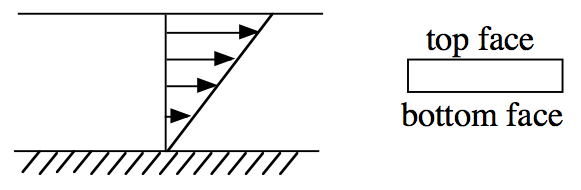
\includegraphics[width=0.6\textwidth]{friction4.png}
	\end{figure}
	\item Top face: $\partial u / \partial z > 0 \rightarrow \tau_{zx} > 0 \rightarrow$ the $x$-component force exerted on the bottom face by the overlying fluid is positive.
	\item The underlying fluid exerts an equal and opposite force on the bottom face via Newton's \nth{3} Law (action/reaction).
	\item This means that the slow fluid underlying the bottom face tries to slow down the faster fluid above it in the parcel.
\end{itemize}
\end{frame}
%------------------------------------------------
\begin{frame}{Conservation of Momentum: Surface Force (Friction)}
\begin{figure}
		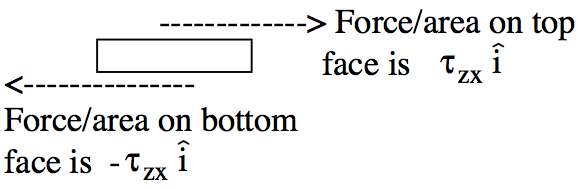
\includegraphics[width=0.6\textwidth]{friction5.png}
	\end{figure}
\begin{itemize}
	\item Because $u$ varies linearly with height, $\partial u / \partial z$ is spatially constant.
	\item This means that $\tau_{zx}$ is constant $\rightarrow$ the forces on the top and bottom faces are equal and opposite.
	\item The result is that there is no net horizontal force, and thus no horizontal acceleration.
	\item This implies steady-state for this experiment.
\end{itemize}
\end{frame}
%------------------------------------------------
\begin{frame}{Conservation of Momentum: Surface Force (Friction)}
\begin{itemize}
	\item Let's move beyond the simple plate experiment and consider a unidirectional shear flow in which $u(z)$ is not linear.
	\item In this case, $\tau_{zx}$ is not spatially constant $\rightarrow$ no steady-state.
	\begin{figure}
		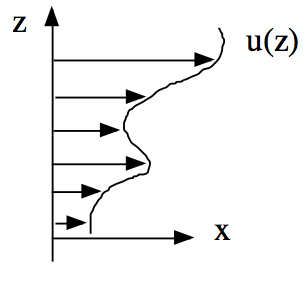
\includegraphics[width=0.6\textwidth]{friction6.png}
	\end{figure}
\end{itemize}
\end{frame}
%------------------------------------------------
\begin{frame}{Conservation of Momentum: Surface Force (Friction)}
\begin{itemize}
	\item Consider an infinitesimally small box of fluid with sides in the $x$, $y$, and $z$ directions of length $\delta x$, $\delta y$, and $\delta z$.
	\begin{figure}
		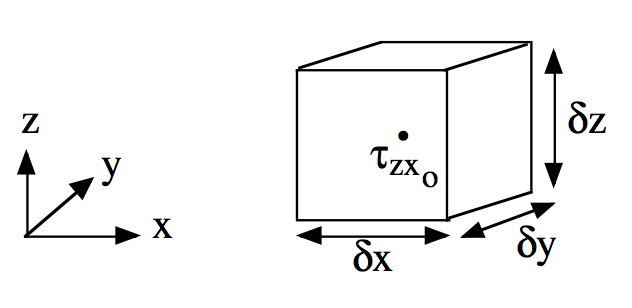
\includegraphics[width=0.8\textwidth]{friction7.png}	
	\end{figure}
	\item $\tau_{zx0}$ is the $x$-component of shearing stress at the center of the box.
\end{itemize}
\end{frame}
%------------------------------------------------
\begin{frame}{Conservation of Momentum: Surface Force (Friction)}
\begin{figure}
		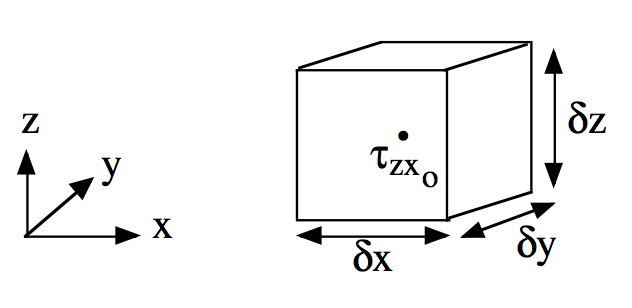
\includegraphics[width=0.6\textwidth]{friction7.png}	
	\end{figure}
\begin{itemize}
	\item The $x$-component of shearing stress at the top of the box is:
	$$\tau_{zx0} + \frac{\partial \tau_{zx}}{\partial z}\frac{\delta z}{2}$$
	\item The $x$-component viscous force on the top face exerted by the overlying fluid is:
	$$\left( \tau_{zx0} + \frac{\partial \tau_{zx}}{\partial z} \frac{\delta z}{2}\right)\delta x \delta y$$
\end{itemize}
\end{frame}
%------------------------------------------------
\begin{frame}{Conservation of Momentum: Surface Force (Friction)}
\begin{figure}
		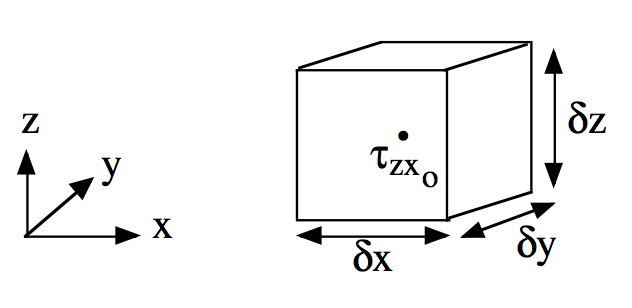
\includegraphics[width=0.6\textwidth]{friction7.png}	
	\end{figure}
\begin{itemize}
	\item The $x$-component of shearing stress at the bottom of the box is:
	$$\tau_{zx0} - \frac{\partial \tau_{zx}}{\partial z}\frac{\delta z}{2}$$
	\item The $x$-component viscous force on the bottom face exerted by the underlying fluid is:
	$$-\left( \tau_{zx0} - \frac{\partial \tau_{zx}}{\partial z} \frac{\delta z}{2}\right)\delta x \delta y$$
\end{itemize}
\end{frame}
%------------------------------------------------
\begin{frame}{Conservation of Momentum: Surface Force (Friction)}
\begin{itemize}
	\item The total $x$-component viscous force on the fluid box is:
	\begin{align*}
	\vv{F_f} &=\left( \tau_{zx0} + \frac{\partial \tau_{zx}}{\partial z} \frac{\delta z}{2}\right)\delta x \delta y -\left( \tau_{zx0} - \frac{\partial \tau_{zx}}{\partial z} \frac{\delta z}{2}\right)\delta x \delta y\\
	&= \frac{\partial \tau_{zx}}{\partial z}\delta x \delta y \delta z
	\end{align*}
	The total $x$-component viscous force per unit mass is:
	\begin{align*}
		F_x &= \cfrac{\cfrac{\partial \tau_{zx}}{\partial z}\delta x \delta y \delta z}{\rho \delta x \delta y \delta z} = \frac{1}{\rho}\frac{\partial \tau_{zx}}{\partial z} = \frac{1}{\rho}\frac{\partial}{\partial z}\left(\mu \frac{\partial u}{\partial z}\right)\  \text{assume $\mu$=contant}\\
		&= \frac{\mu}{\rho}\frac{\partial^2 u}{\partial z^2}\\
		&= \nu \frac{\partial^2 u}{\partial z^2}
	\end{align*}
	where $\nu = \mu / \rho$ is kinematic viscosity.
\end{itemize}
\end{frame}
%------------------------------------------------
\begin{frame}{Conservation of Momentum: Surface Force (Friction)}
\begin{itemize}
	\item In reality, $u$ will vary in the $x$, $y$, and $z$ directions $\rightarrow$ $u = u(x,y,z)$. Thus, 
	\begin{align*}
	\frac{F_x}{m} &= \nu \left(\frac{\partial^2 u}{\partial x^2} + \frac{\partial^2 u}{\partial y^2} + \frac{\partial^2 u}{\partial z^2}\right) = \nu \vv{\nabla}^2 u
	\end{align*}
	In general, there are also $v=v(x,y,z)$ and $w=w(x,y,z)$ components to consider:
	\begin{align*}
	\frac{F_y}{m} &= \nu \left(\frac{\partial^2 v}{\partial x^2} + \frac{\partial^2 v}{\partial y^2} + \frac{\partial^2 v}{\partial z^2}\right) = \nu \vv{\nabla}^2 v\\
	\frac{F_z}{m} &= \nu \left(\frac{\partial^2 w}{\partial x^2} + \frac{\partial^2 w}{\partial y^2} + \frac{\partial^2 w}{\partial z^2}\right) = \nu \vv{\nabla}^2 w
	\end{align*}
	or in vector form:
	$$\frac{\vv{F_f}}{m} = \boxed{\nu \left(\frac{\partial^2 \vv{u}}{\partial x^2} + \frac{\partial^2 \vv{u}}{\partial y^2} + \frac{\partial^2 \vv{u}}{\partial z^2}\right) = \nu \vv{\nabla}^2 \vv{u}}$$
\end{itemize}
\end{frame}
%------------------------------------------------
\begin{frame}{Conservation of Momentum: Surface Force (Friction)}
\begin{itemize}
	\item The physical basis for viscous force in the atmosphere is the random migration of air molecules.
	\item Consider a large-scale flow where $u$ increases with height.
	\item Downward-moving molecules have larger $u$ than upward-moving molecules.
	\item Thus, faster momentum is brought down and slower momentum is moved upward (mixing) $\rightarrow$ bigger $\partial u / \partial z$ means greater momentum transport by frictional effects.
	\item Is the net effect dominated by downward or upward momentum transport? This is determined by the vertical derivative ($\partial / \partial z$) of the shear ($\partial u / \partial z$).
\end{itemize}
\end{frame}
%------------------------------------------------
\begin{frame}{Conservation of Momentum: Surface Force (Friction)}
\begin{itemize}
	\item The origin of friction in liquids is much more complicated. 
	\item There is some attraction between molecules, but not much in the way of migration.
	\item Notably, we get the same mathematical description of the viscous force as for gases ($\vv{F_f} = \nu \vv{\nabla}^2 \vv{u}$) - just with a different value for $\nu$.
	\item However, for $T\uparrow$ we get that $\nu_{\text{water}} \downarrow$ and $\nu_{\text{air}} \uparrow$.
\end{itemize}
\end{frame}
%------------------------------------------------
\end{document}

